\documentclass[10pt,conference,compsocconf]{IEEEtran}

\usepackage[hidelinks]{hyperref}
\usepackage{tikz}
\usepackage{float}
\usepackage{algorithm}
\usepackage{algcompatible}
\usepackage{graphicx}	% For figure environment
\usepackage{amsmath} % for mathematical symbols and environments
\usepackage{amssymb} % for mathematical symbols
\usepackage{amsfonts} % for mathematical fonts
\usepackage{bbm} % for blackboard bold symbols
\usepackage{setspace} % for blackboard bold symbols

\algdef{SE}[SUBALG]{Indent}{EndIndent}{}{\algorithmicend\ }%
\algtext*{Indent}
\algtext*{EndIndent}

\begin{document}
\title{Loadboi: An Adaptive Load Generator for Testing Online Services}

\author{
  Emilien Guandalino, Clément Charmillot\\
  \textit{École Polytechnique Fédérale de Lausanne, Switzerland}
}

\maketitle

\begin{abstract}
	When testing online services, researchers often need to evaluate the maximum throughput under a given tail latency requirement. Currently, this is done manually which is tedious and unproductive work. Furthermore, this method does not give any guarantee of optimality for its output. In this project, we propose an adaptive load generator which aims to find maximal throughput under tail latency constraint for online services. We detail our solution's design and present its evaluation. We find that our algorithm is able to maximize the throughput under tail latency constraint within minutes of execution time.

\end{abstract}

\section{Introduction} \label{intro}

In 2006, Amazon published a remarkable statistic: every added 100ms of latency in page load time cost them 1\% of annual revenue, equating to around \$3.8 billions today. As a consequence of this realization, reducing latency has become a central concern in online services. Service Level Objectives (SLOs) enforce tight tail latency constraints to ensure that an overwhelming majority of requests, ex: 99\%, are served within a certain response time. When evaluating those online services in a research environment, one of the main goals is to find highest throughput one can achieve within the tail latency constraint. However, this evaluation is currently done manually, meaning that the researcher goes through an iterative process of: 1) running the workload for a certain throughput, 2) waiting for an arbitrary period of time and 3) measuring the tail latency to see if the SLO is respected. This cumbersome work may take hours, and at the end of this painful process, the researcher has no guarantee that his result is optimal. Our work aims to provide a solution to this problem by designing and implementing an adaptive load generator which provably finds the maximal throughput under SLO constraint for an online service.

This rest of this report is organized as follows: section \ref{background} gives background on the nature of tail latency and provides insights on why our task is challenging. Section \ref{prior} lists existing relevant work and states their relation with our work. Section \ref{contr} gives an overview of our contribution. Section \ref{design} details the design of our solution. Section \ref{eval} outline the methodology and results of our evaluation. Section \ref{future} gives directions for future improvements and section \ref{sum} summarizes our work.

\section{Background} \label{background}

Latency in online services stems from a variety of unpredictable factors such as network queuing delays, OS intervention, garbage collection and many more. By nature, latency is a volatile metric and even more so when looking at tail latency, i.e. the higher percentiles of the latency distribution.

This variability can be observed even for a constant load in Figure \ref{fig:lat1}, using a log scale.
\begin{figure}[H]
	\centering
	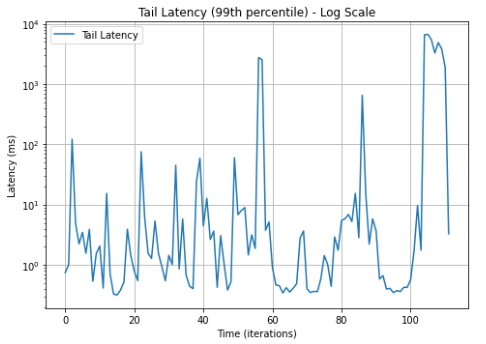
\includegraphics[width=0.4\textwidth]{lat.png}
	\caption{Tail Latency at constant load}
	\label{fig:lat1}
\end{figure}

In addition to having a large baseline variance, tail latency also has sporadic peaks which deviate exponentially more than average. Those peaks make our task particularly challenging as they are unpredictable and may cause the service to break the tail latency SLO. This is true at constant load but even more so when increasing the load. Figure \ref{fig:lat2}. shows tail latency as we progressively increase the load, marked by the dashed green vertical lines.

\begin{figure}[H]
	\centering
	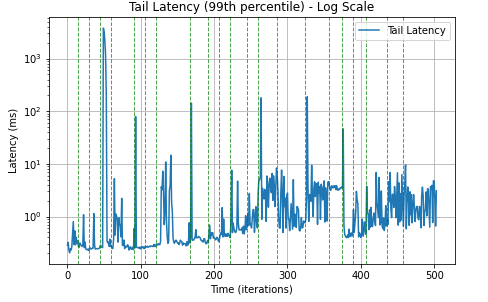
\includegraphics[width=0.45\textwidth]{lat2.png}
	\caption{Tail Latency at increasing loads}
	\label{fig:lat2}
\end{figure}

As we can see, those effects are exacerbated at high throughput.  Furthermore, we can also notice that tail latency is sensitive to workload changes, and some of the peaks are directly caused by performing an increase in workload. Making a change in such a complex system adds oil to the fire, and results in more exponential peaks. 

Designing an algorithm whose purpose is to maximize load under a tail latency constraint is therefore a challenging task and is the object of our work.

\section{Prior Work}\label{prior}

Tail Latency has been the object of research for many years and multiple works revolve around finding its causes and accurately measuring it. To cite just a few, works such as CloudSuite \cite{clouds} and Tailbench \cite{tailbench} provide a benchmark suite for evaluating latency in online services. Treadmill \cite{treadmill} further proposes a framework for attributing latency to different factors. 

Concerning load generators, works such as In-Vitro \cite{in-vitro} use production traces to generate loads which accurately represents production environments. We should note that our purpose here is different from such type of works, as we are in a testing environment where we have full control over the throughput and are attempting to maximize it. 

To realize this project, we build on top of the abstraction of a framework which provides realistic request generation and precise latency measurement. Our work is parallel to other load generators such as In-Vitro, as it serves a different purpose and makes different assumptions.

\section{Contribution}\label{contr}

We devise and evaluate an algorithm for throughput maximization under a given tail latency constraint. There are multiple design goals which have guided our decisions when implementing the algorithm. Those goals are as follows:

\begin{enumerate}
	\item \textit{Precision and Execution Time}: There is a tradeoff between the precision of the algorithm's output, and its total execution time. Our goal is to be able to produce results with satsisfying precision in a reasonable amount of time, i.e. not exceeding a few hours. The researcher should also be able to require arbitrarily precise results, if he is willing to run the algorithm for a longer time.

	\item \textit{General Purposed}: We should not require the researcher to adapt the logic of the algorithm for each specific workload. Ideally, the algorithm should be agnostic of the underlying framework, by assuming a simple API which all workloads can comply to. As a result, we have designed our algorithm to only model tail latency as a univariate function of throughput.

	\item \textit{Output Guarantees}: We want the output of the algorithm to satisfy certain properties, for example statistical certitude of correctness and optimality guarantees. More details will be given in the next section as to how we achieve this.
\end{enumerate}

Figure \ref{fig:layers}. shows at which layer our algorithm operates. Our algorithm assumes a simple API from the layer underneath, and makes requests of the form:

\vspace{0.5em}
\noindent [\textit{Latencies}] \textbf{sample\_requests} (\textit{num\_requests, QPS})
\vspace{0.5em}

The function \textbf{sample\_requests} takes as input the number of requests to perform and a throughput, for example in the form of a Query Per Second (QPS) rate. It then returns a list of latencies of size \textit{num\_requests} corresponding to the latency of each request.

\begin{figure}[H]
	\centering
	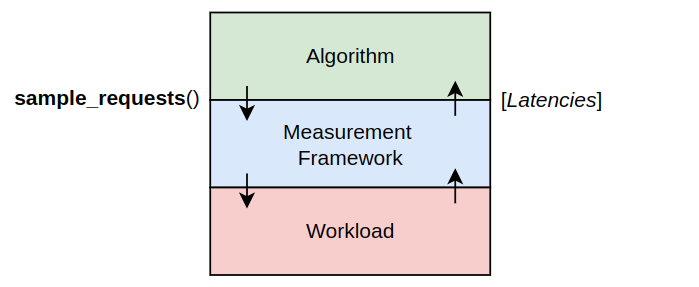
\includegraphics[width=0.5\textwidth]{layers.png}
	\vspace{-1em}
	\caption{Layer hierarchy}
	\label{fig:layers}
\end{figure}

As mentioned previously, we build on top of the abstraction of a framework which will perform those requests for us, and output the latencies. This means that our algorithm is portable to any framework which can provide this simple API call. We now give more details on the design of the algorithm.

\section{Design}\label{design}


From a high level perspective, the algorithm is simple and its description fits in a few line. This is a direct consequence of our goal to keep it general purpose and restricting its possible actions to 1) measuring tail latency and 2) performing a workload change. The main difficulty in our situation is providing rigorous guarantees on its output. We have designed the algorithm to provide two properties:

\begin{enumerate}
	\item \textit{Correctness}: As we are working with a volatile metric, tail latency, we need to ensure that our estimates are correct. This can be achieved by using statistical tools which tell us how many requests we should make in order to accurately estimate latency, depending on the desired confidence interval.

	\item \textit{Optimality}: Since we are performing changes in a complex system, and by the nature of latency which comes from a range of different factors, the underlying distribution that we are estimating is also changing over the course of time. We therefore need to ensure that we have actually converged before taking a decision.
\end{enumerate}

At the end of the execution, the output of the algorithm is guaranteed to be correct, i.e. close to the SLO (up to an error term) with the desired statistical certainty, and optimal, meaning that the output value is one to which the algorithm has converged. 

The algorithm description is given in Alg. \ref{alg:cap}. For each iteration, 3 main tasks are performed . The first one determines the size of the sampling window in order to perform the correct amount of requests. The second task detects convergence, both locally and globally. The third task performs the change in workload.

\begin{algorithm}
	\caption{Load-Aware Load Generator}\label{alg:cap}
	\begin{algorithmic}[1]
		\STATE \textbf{repeat:}
		\Indent
		\STATE n $\gets$ sampling\_window()
		\STATE sample\_requests(n, QPS)
		\STATE latency $\gets$ aggregate\_latencies()
		\STATE converged $\gets$ local\_convergence(latency) 
		\IF{converged}
		\IF{ global\_convergence(latency, SLO)} 
		\STATE \textbf{return} (load, latency)
		\ELSIF{latency $<$ latency\_requirement}
		\STATE QPS = increase\_load(QPS) 
		\ELSIF{latency $>$ latency\_requirement}
		\STATE QPS = decrease\_load(QPS)
		\ENDIF
		\ENDIF
		\EndIndent
	\end{algorithmic}
\end{algorithm}


\subsection{Sampling Window}

To ensure correctness of our result, we need to have some statistical certainty about the estimates that we produce. The minimum size of the request sample is given as follows:

\begin{align*}
	n = Z^2\frac{\text{Var}(\hat{Q})}{\epsilon^2}
\end{align*}

where $\hat{Q}$ is the estimate of the distribution of request latencies, $\epsilon$ is the error term from which we are willing to deviate from the true mean, and $Z$ is the $Z$-score associated with the confidence interval, for example 1.96 for 95\% percentile. Our algorithm determines this sample size at each iteration and decides to increase the load or output a result only if enough requests have been made. 

Not only does this ensure correctness of the outputs, it also improves the running time. Unlike manually adjusting the load, where the researcher has to wait for an arbitrary amount of time, we know exactly how many samples we need to produce before taking a decision. This greatly speeds up the process of finding a maximum.

\subsection{Convergence Detection}

Convergence is detected at two levels: locally and globally. Local convergence ensures that we have converged to a distribution before we take a decision. Global convergence detects when we have locally converged to a value which is close enough from the target SLO.

To ensure the optimality of our solution, we check for local convergence before every decision, including when outputing a value, so that we do not return a value while the distribution of the latency is still changing. We do this by evaluating the coefficient of variance  over a set window of samples.

\begin{align*}
	CV := \frac{\sigma}{\hat{E}}
\end{align*}

The coefficient of variance will measure how much the values within a window are concentrated around their mean. In the case of a converging sequence, such as on Figure \ref{fig:cv}, a larger coefficient of variance will accept larger deviation in the sequence and therefore would detect convergence at a point where the slope of the tangent is not entirely flat. When choosing this variation coefficient, there is once again a tradeoff between precision and speed of the algorithm. If the coefficient is too high, we may detect convergence and output a result which is not optimal, i.e. could be improved or one that would break SLO requirement if given more time. If the coefficient is too low, upon each iteration, we will require an even larger amount of requests to dampen small variations and finally converge.

\begin{figure}[H]
	\centering
	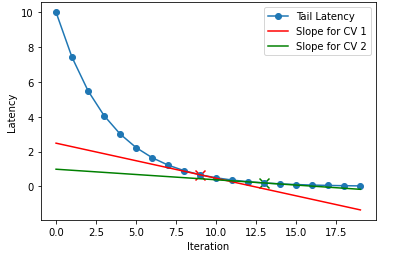
\includegraphics[width=0.45\textwidth]{CV.png}
	\caption{Converging points according to different CVs}
	\label{fig:cv}
\end{figure}

After discussion during the poster session, it was mentioned to us that microservices sometimes have a slow cascade of latency which takes time to propagate. To detect such fine grained divergence, the coefficient of variance should be very small.

There is also a choice in the window size that we consider for convergence. This can be used if we want to forget previous "bad" behavior after a certain amount of time.

\subsection{Workload Updates}

Once the algorithm is certain that the latency it is measuring is both correct and has converged to a value below the SLO, it can decide to increase the load. The new load takes into account the distance to the SLO. This ensures faster progress when we are far from the objective, and finer grained progress when we are close. The updates are also clamped to avoid performing too big changes in a single step, which can increase the variance too much and delay convergence. Some damping also prevents oscillations around the target SLO and helps to accelerate the convergence. 

In order to account for the variability caused by a change in workload, we have added a small warmup window after each change, during which latency is not observed.

\section{Evaluation} \label{eval}

\subsection{Methodology}

We ran our experiments using the Tailbench benchmark suite. We ran the TPC-C benchmark, an Online Transaction Processing (OLTP) benchmark, on Silo database. We ran in integrated configuration, meaning that all requests happened in memory. All experiments were performed on our machines.

To estimate the latency distribution, we used histograms of request as they are a convenient and memory efficient way to accurately aggregate latencies. As inputs, our algorithm is given a target SLO, an error tolerance, a tail latency percentile, the variation coefficient limit and the confidence interval parameters.

\subsection{Results}

We now give the results of our evaluation. We can see in figure \ref{fig:res1}. that the latency is slowly increased until it reaches the SLO requirement where it detects convergence and outputs the result.

\begin{figure}[H]
	\centering
	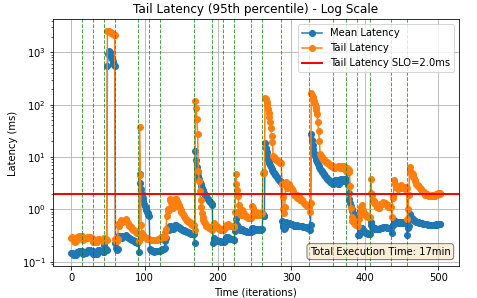
\includegraphics[width=0.5\textwidth]{result1.png}
	\vspace{-1em}
	\caption{SLO: 2ms, Error Tolerance: 0.2ms}
	\label{fig:res1}
\end{figure}

Figure \ref{fig:res2}. shows another experiment where the variance was much greater. There can be multiple explanations for this, such as the fact that we are targetting a smaller SLO, or due to different background activities on the machine. The graph is more chaotic, but the algorithm is still able to maximize the throughput.

\begin{figure}[H]
	\centering
	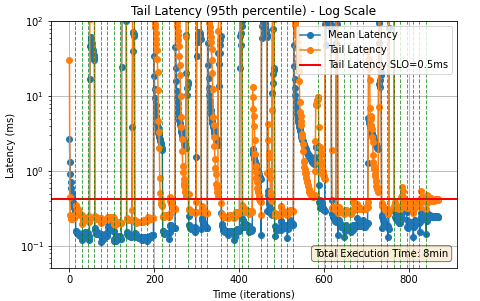
\includegraphics[width=0.5\textwidth]{result2.png}
	\vspace{-1em}
	\caption{SLO: 0.5ms, Error Tolerance: 0.1ms}
	\label{fig:res2}
\end{figure}

We can see that the algorithm converged quicker in this case, despite a smaller target SLO. We believe this to be due to the fact that the ratio of the error tolerance compared to the target SLO is larger here (0.1ms to 0.5ms compared to 0.2ms to 2ms), and so the precision requirement is actually lower in the second case.

Overall, the algorithm is able to maximize the throughput within minutes, even for small SLOs. This however depends on the tuning of the parameters which we mentioned previously. 

Concerning the target SLOs of our experiments, it was not possible to obtain results for greater values on our machines. At low throughput, increasing the load also increases the tail latency somewhat linearly, but after a certain kneecap point, it explodes to exponentially large values because of saturation. This transition is very sharp and although we were able to target SLOs of around 2ms, we were not able to get results for higher SLOs, as the tail latencies would immediately explode to thousands of ms. The algorithm would then oscillate between 2-4ms and thousands of ms. Furthermore, since this caused great variance, the required sample sizes for accurate measurement were huge and prevented convergence within a reasonable amount of time. 

We do not believe that this is an inherent problem of our algorithm, but more one of the choice of the SLO. We cannot see any situation were it is desirable to be at the edge of this kneecap saturation point such that any variation in load might explode the tail latency and break all requirements.


\section{Future Work}\label{future}

Much work remains in fine tuning the algorithm and increasing its robustness. This could be achieved by testing it on different workloads, such as memcached, and in different configurations, for example in a networked configuration. Since the algorithm is general purposed, it should also be able to target different SLO ranges, from microsecond to second. There is also the problem of "performance hysteresis" which needs to be addressed. Performance hysteresis refers to the fact that a given throughput might converge to different tail latencies in different executions. This is due to variations in initial configurations and other randomness during runtime, which are out of our control. A proposed solution is to run multiple executions and average across them. Our algorithm currently only optimizes within a single run, but multiple runs might produce different results, due to the nonconvexity of the problem.

\section{Summary} \label{sum}

In summary, we have presented and evaluated a load aware load generator for testing online services. Our solution builds on top of the abstraction of a latency measurement framework, and provides guarantees of correctness and optimality for its solutions. In our evaluation, we have demonstrated that our algorithm is able to find a maximum throughput under SLO constraint within minutes.

\section*{Acknowledgements}
We would like to thank the CS-471 teaching staff for their precious help and advice in the early stages of the project. In particular, we would also like to thank Shanqing for his support and dedication, remaining available well past usual working hours.

\singlespacing
\singlespacing
%\newpage
\bibliographystyle{IEEEtran}
\bibliography{ref}

\end{document}
